\documentclass[9pt]{beamer}

\beamertemplatenavigationsymbolsempty
\renewcommand\mathfamilydefault{cmr}

\usepackage{pajmath}
\usepackage{booktabs}
\usepackage{colortbl}

\usepackage{tikz}
\usetikzlibrary{positioning,shapes.misc,calc,backgrounds,scopes} 
\usetikzlibrary{datavisualization}
\usetikzlibrary{datavisualization.formats.functions}
\tikzset{boxed/.style={
  thick,
  draw=black,
  top color=white,
  text height=1.5ex,
  text depth=.25ex
}}


\newcommand\lo{$-1$}
\newcommand\hi{$\phan1$}
\newcommand\ze{$\phan0$}
\newcommand\Ze{$\phan\Vzero$}
\newcommand\pskip{\pause\bigskip}
\newcommand\lspace{\addtolength{\itemsep}{0.5\baselineskip}}
\newcommand\red[1]{{\color{red}#1}}

\title{Reinforcement Learning:\\Rollout}
\author{BIOE 498/598 PJ}
\date{Spring 2021}

\begin{document}
\frame{\titlepage}

\begin{frame}{Review}

The \emph{value function} is the expected sum of future rewards
\[ V(s_i) = \mathbb{E}\{ r_i + r_{i+1} + \cdots + r_T \}. \]

\bigskip
At any state $s_i$, the optimal policy follows the objective
\begin{align*} 
	 & \max_{a_i} \mathbb{E}\{ r_i + r_{i+1} + \cdots + r_T \} \\
	=& \max_{a_i} \mathbb{E}\{r_i\} + \mathbb{E}\{r_{i+1} + \cdots + r_T \} \\
	=& \max_{a_i} \mathbb{E}\{r_i\} + V(s_{i+1})
\end{align*}

\end{frame}

\begin{frame}{Optimal policies can be found with a value function.}

The optimal RL policy balances the immediate reward $r_i$ with future rewards $V(s_{i+1})$:
	\[ \pi^*(s_i) = \arg \max_{a_i}\left\{ \mathbb{E}[r_i] + V(s_{i+1}) \right\}. \]
	
\pskip
If we know the value function, the optimal policy is to be greedy with respect to it. However, we rarely know $V$:
\begin{itemize}
	\item Monte Carlo estimation of $V$ is only approximate even with many simulations.
	\item If the state space is very large, we may never visit every state to estimate $V$ by tabular methods.
\end{itemize}

\pskip
Instead, we use an \emph{approximate value function} $\widetilde{V}(s)$ to find a sub-optimal policy $\pi(s)$.
\end{frame}

\begin{frame}{Approximate value functions.}
There are two classes of methods for approximating a value function.
\bigskip

\begin{enumerate}\lspace
	\item \textbf{Parametric approximation} trains a model that predicts value from previous visits to states. The model predicts the value for \emph{all} states, even those that have not been visited.
	\begin{itemize}
		\item Any type of model can be used to predict value: Linear models, Gaussian Process Regression, Artificial Neural Networks (``Deep RL'').
		\item Parametric methods are often \emph{offline}; the model is trained before the agent uses the model to navigate an MDP.
	\end{itemize}
	\pause
	\item \textbf{Monte Carlo approximation} uses a model of the MDP to simulate the rewards following a state.
	\begin{itemize}
		\item Monte Carlo methods work well \emph{online} by simulating states just ahead of the agent in the MDP.
		\item These methods are \emph{sample efficient} but require a computational model of the MDP.
	\end{itemize}
\end{enumerate}
	
\end{frame}

\begin{frame}{Rollout}

\begin{itemize}\lspace
	\item Rollout is a Monte Carlo method frequently used for online RL.
	\item Rollout ``looks ahead'' to estimate the value of states the agent is likely to visit next.
	\item Rollout is robust and works with many RL problems. Variants of rollout (e.g.\ MCTS) power AlphaGo, AlphaZero, and other top game engines.
	\item Rollout can be used for policy iteration, but we will limit our discussion to a single pass through an MDP.
\end{itemize}
	
\end{frame}

\begin{frame}{The rollout algorithm}

Rollout requires 
\begin{itemize}
	\item A \emph{simulator} that generates sequences \[ s_i,a_i,r_i,\ldots,s_{T-1},a_{T-1},r_{T-1},\,s_T,r_T \] given a policy $\pi$.
	\item A \emph{base policy} $\pi_\text{base}$ to use with the simulator. A random base policy works.
\end{itemize}

\begin{center}
	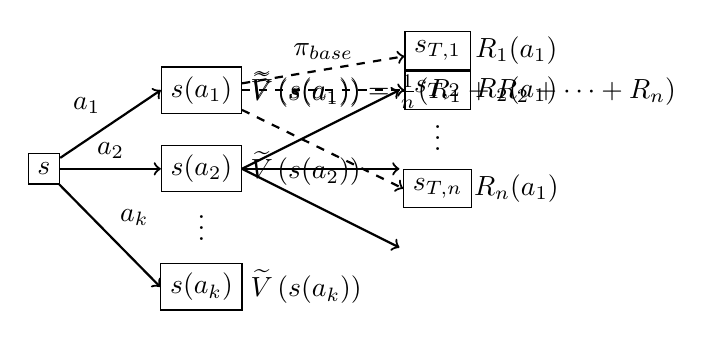
\begin{tikzpicture}
		\onslide<2->{
			\node [draw] (si) at (0,0) {$s$};
		}
		\onslide<3-7>{
			\node [draw] (si1) at (2,1) {$s(a_1)$};
			\draw [->,thick] (si) -- (si1.west) node [midway,above left] {$a_1$};
		}
		\onslide<4-5>{
			\node [draw] (sT1) at (5,1.5) {$s_{T,1}$};
			\node [draw] (sT2) at (5,1) {$s_{T,2}$};
			\node (sTe) at (5,0.5) {$\vdots$};
			\node [draw] (sTn) at (5,-0.25) {$s_{T,n}$};
			\draw [->,thick,dashed] (si1) -- (sT1) node [midway,above] {$\pi_\text{base}$};
			\draw [->,thick,dashed] (si1) -- (sT2);
			\draw [->,thick,dashed] (si1) -- (sTn.west);
		}
		\onslide<5-5>{
			\draw (6,1.5) node {$R_1(a_1)$}
			  	  (6,1) node {$R_2(a_1)$}
			  	  (6,-0.25) node {$R_n(a_1)$};
		}
		\onslide<6-6>{
			\draw (si1) ++(0.5,0) node [right] {$\widetilde{V}\left(s(a_1)\right) = \frac{1}{n}(R_1 + R_2 + \cdots + R_n)$};
		}
		\onslide<7->{
			\node [draw] (si2) at (2,0) {$s(a_2)$};
			\draw [->,thick] (si) -- (si2.west) node [midway,above] {$a_2$};
		}
		\onslide<7-7>{
			\node (sie) at (2,-0.65) {$\vdots$};
			\node [draw] (sik) at (2,-1.5) {$s(a_k)$};
			\draw [->,thick] (si) -- (sik.west) node [midway,above right] {$a_k$};
			\draw (si1) ++(0.5,0) node [right] {$\widetilde{V}\left(s(a_1)\right)$};
			\draw (si2) ++(0.5,0) node [right] {$\widetilde{V}\left(s(a_2)\right)$};
			\draw (sik) ++(0.5,0) node [right] {$\widetilde{V}\left(s(a_k)\right)$};
		}
		\onslide<8->{
			\draw [thick,->] (si2.east) -- ++(2,1);
			\draw [thick,->] (si2.east) -- ++(2,0);
			\draw [thick,->] (si2.east) -- ++(2,-1);
		}
	\end{tikzpicture}
\end{center}

\end{frame}

\begin{frame}{Rollout in Gridworld}

\begin{columns}
\begin{column}{0.4\textwidth}
	\begin{center}
		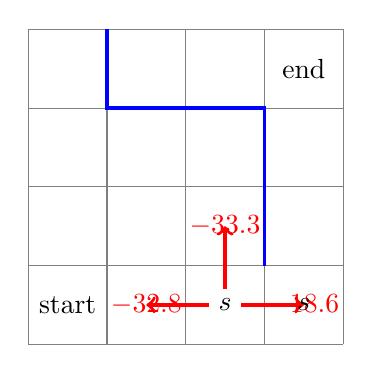
\begin{tikzpicture}[scale=1]
			\draw [color=gray,thin] (0,0) grid (4,4);
			\node at (0.5,0.5) {start};
			\node at (3.5,3.5) {end};
			\draw [very thick,blue] (1,4) -- (1,3) -| (3,1);
			\onslide<1-3>{
				\node (s) at (2.5,0.5) {$s$};
			}
			\onslide<2-2>{
				\draw [very thick,red,->] (s) -- ++(-1,0);
				\draw [very thick,red,->] (s) -- ++(1,0);
				\draw [very thick,red,->] (s) -- ++(0,1);
			}
			\onslide<3-3>{
				\draw [red] (s) ++(-1,0) node {$-32.8$}
					  (s) ++(0,1) node {$-33.3$}
					  (s) ++(1,0) node {$-18.6$};
			}
			\onslide<4->{
				\draw (3.5,0.5) node {$s$};
			}
		\end{tikzpicture}
	\end{center}
\end{column}

\begin{column}{0.6\textwidth}
	\begin{itemize}
		\item Imagine we are in the middle of the maze at state~$s$.
		\item<2-> There are three available actions: \{left, up, down\}.
		\item<3-> We use random walks to estimate $\widetilde{V}$ after each action.
		\item<4-> We select the action that leads to the best estimated value.
	\end{itemize}
\end{column}
\end{columns}
	
\end{frame}

\begin{frame}{Policy improvement with rollout}

\begin{itemize}\lspace
	\item The online policy we are finding is called the \emph{rollout policy}.
	\item The rollout policy has the \emph{policy improvement property} --- it will be equal to or better than the base policy.
	\item We can repeat the process with another trip through the MDP using the rollout policy as the new base policy.
	\item However, iterating in this way requires us to add exploration to our policies.
\end{itemize}
	
\end{frame}


\begin{frame}{Summary}

\begin{itemize}\lspace
	\item \textbf{Rollout} is an online method that reduces simulation by focusing on local starts.
	\item A single pass with a random base policy provides good, but not necessarily optimal, behavior.
	\item Iteration and exploration are required to find optimal policies.
\end{itemize}

\end{frame}

\end{document}
